\section[Welcome from Prof. Yoshio Hisaeda]{Welcome message from the Dean of Engineering at Kyushu University, Prof. Yoshio Hisaeda}

\begin{wrapfigure}{r}{0.25\textwidth}
    \begin{center}
        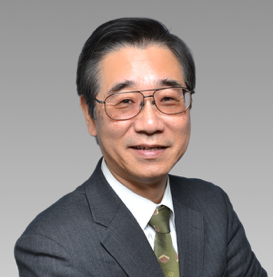
\includegraphics[width=0.23\textwidth]{hisaeda.png}
    \end{center}
\end{wrapfigure}

I am delighted to welcome you to the 6th UK-Japan Engineering Education League Workshop, held for the first time at Kyushu University. Given the long history of academic collaboration between the UK and Japan in fields of engineering education and research which extends back more than 150 years, this event represents a important continuation of cultural and scientific exchange for current and future generations of scientists, and we are proud to be the hosts of the 6th UKJEEL workshop.
 
The Faculty of Engineering in Kyushu University is the fourth oldest faculty among Japanese universities, and was founded as the College of Engineering of Kyushu Imperial University in 1911. Since that time, as one of the key faculties of the leading universities in Japan, the faculty has contributed to the development of engineering, technology and industry in Japan and worldwide, providing leading research and enhanced engineering education. This year is particularly momentous: the ceremony to celebrate completion of our new campus ``Ito Campus'' is being held this September.

I hope you all take this opportunity to build personal and professional connections between the Japanese and the UK scientific communities, and that your visit to Kyushu University and the wider Fukuoka region is an interesting and enjoyable one.

\vspace{1em}
\noindent Yoshio Hisaeda\\
Kyushu University\\
Dean of Engineering


\newpage
\section[Welcome from Prof. Roderick A Smith]{Welcome message from the Chair of UKJEEL, Prof. Roderick A Smith}

\begin{wrapfigure}{r}{0.25\textwidth}
    \begin{center}
        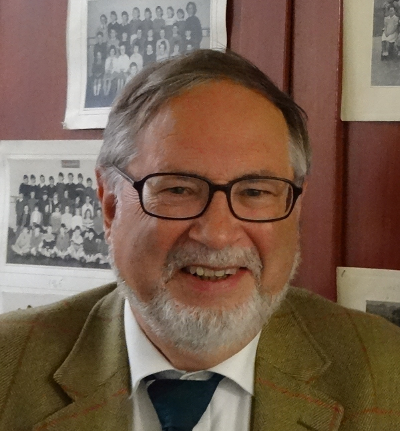
\includegraphics[width=0.23\textwidth]{smith.png}
    \end{center}
\end{wrapfigure}

I am delighted to welcome you to the 6th UK-Japan Engineering Education League Workshop, held for the first time at Kyushu University. Given the long history of academic collaboration between the UK and Japan in fields of engineering education and research which extends back more than 150 years, this event represents a important continuation of cultural and scientific exchange for current and future generations of scientists, and we are proud to be the hosts of the 6th UKJEEL workshop.
Welcome to Kyushu and its great university! 

Kyushu has been known throughout the history of Japan as a international gateway with particularly close links to Korea and China and, of course, the tiny trading island of Dejima in Nagasaki which maintained trading with the European nations even though the long period when Japan was officially closed.
 
In the next few days, during the 6th UK Japan Engineering Education League (UKJEEL) workshop, we are going to explore modern issues of materials engineering and the ways it might contribute to building a better earth in the future. To our young students here is an opportunity to become involved in the great issues which face us: Important because our future is in the hands of you and your colleagues all over the world, the engineers of the future. To our older faculty colleagues we will demonstrate that learning is a lifelong process and we discuss ideas to improve our teaching and enrich the learning experience we offer to our students. But we also have time to explore togther the delights of Kyushu, old and new. 

Kyushu University has a very strong international engineering presence. I am sure you will return home having fallen in love with this magical part of Japan: the interplay between sea and mountains, the wonderful food, the onsens and, of course, the warm and hospitable people.

Enjoy Kyushu and UKJEEL 2018!

\vspace{1em}
\noindent Roderick A Smith\\
Imperial College London\\
Chair UKJEEL

